\subsection{Package \lstinline!cryptocast.comm!}
This package provides functionality related to communication between the different layers
 of the network protocol and to the communication between the server and clients. This includes
 the management of file and socket streams and abstractions of the multi-client unidirectional
 streams that represent the core of this project.
 Useful abstractions for layered protocols are also included.

\noindent\begin{minipage}[t]{5cm}
\vspace{0.3em}
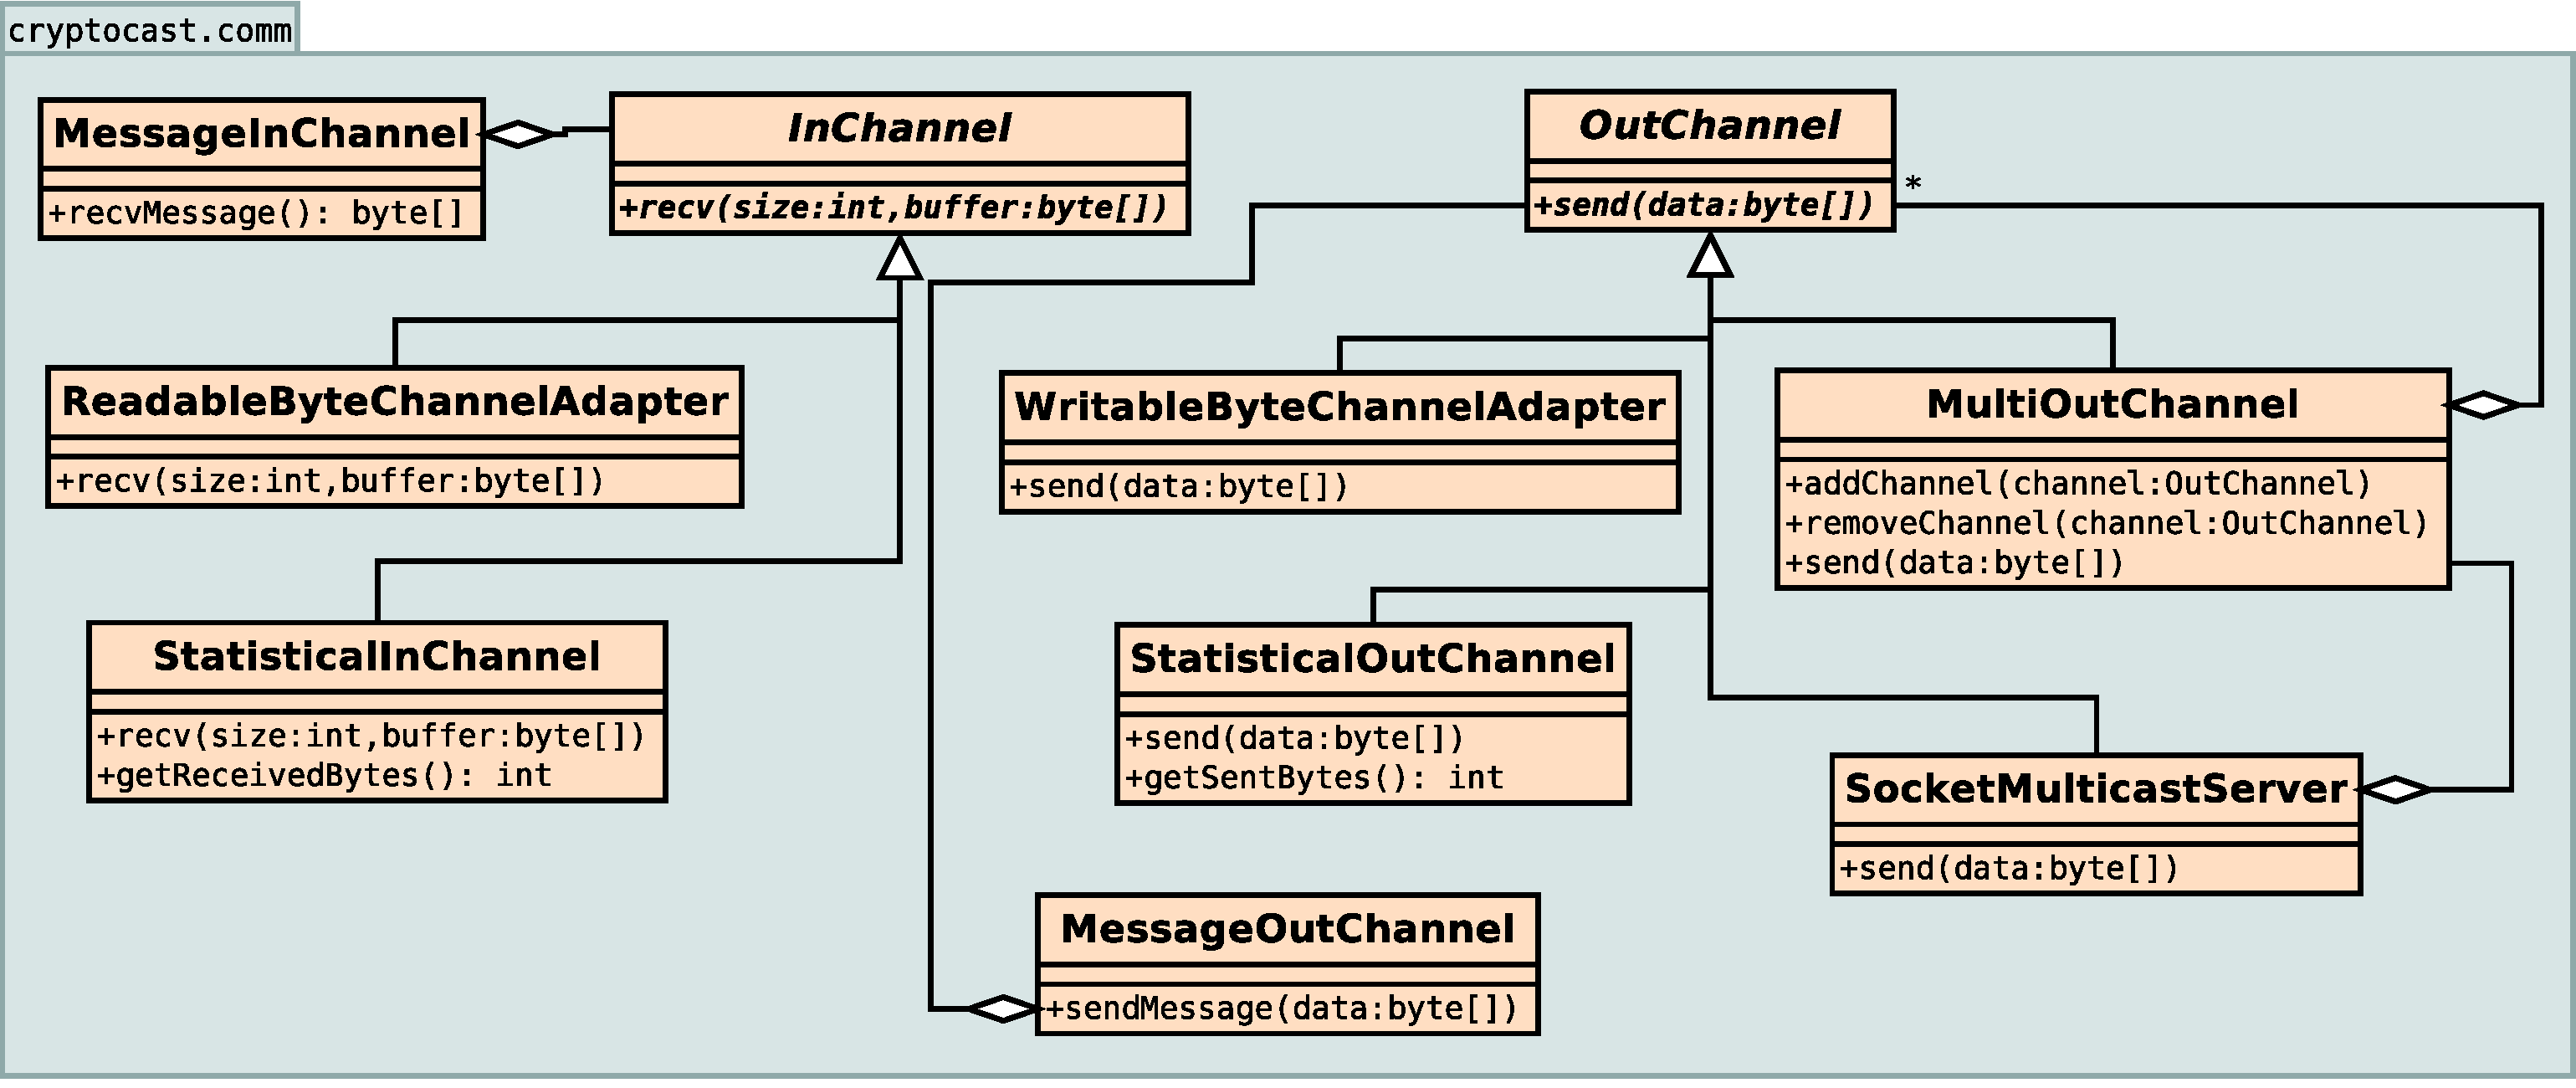
\includegraphics[width=450px]{class_diagrams/cryptocast_comm.pdf}
\end{minipage}

\subsubsection{Class \lstinline|MultiOutputStream|}
Multiplexes several instances of \lstinline|OutputStream|s so that they can be used as a single
 destination. \\
\noindent\begin{minipage}[t]{5cm}
\vspace{0.3em}
\hspace*{2em}
\begin{tikzpicture}
\umlclass[]{MultiOutputStream}{

}{
+ getChannels() : ImmutableList<OutputStream> \\
+ addChannel(channel : OutputStream) \\
+ removeChannel(channel : OutputStream) \\
+ write(data : byte[], offset : int, len : int) \\
+ write(b : int)
}
\end{tikzpicture}
\vspace{0.3em}
\end{minipage}



\textbf{\sffamily Superclasses and Interfaces}
\begin{itemize}
\item \lstinline|java.io.OutputStream|
\end{itemize}


\textbf{\sffamily Constructors}
\begin{itemize}
\item \lstinline|public| \lstinline|MultiOutputStream|\lstinline|(ErrorHandler errHandler)|\\ \\[-0.6em]
Creates an instance of MultiOutputStream.
\begin{itemize}
\item \lstinline|errHandler|: An error handler instance.
\end{itemize}



\item \lstinline|public| \lstinline|MultiOutputStream|\lstinline|()|\\ \\[-0.6em]
Creates an instance of MultiOutputStream that passes on all errors to
 the caller.



\end{itemize}


\textbf{\sffamily Methods}
\begin{itemize}
\item \lstinline|public ImmutableList<OutputStream>| \lstinline|getChannels|\lstinline|()|\\ \\[-0.6em]
\emph{Returns:} the list of output channels



\item \lstinline|public void| \lstinline|addChannel|\lstinline|(OutputStream channel)|\\ \\[-0.6em]
Adds the given channel to the list of receivers.
\begin{itemize}
\item \lstinline|channel|: The channel to add
\end{itemize}



\item \lstinline|public void| \lstinline|removeChannel|\lstinline|(OutputStream channel)|\\ \\[-0.6em]
Removes the given channel from the list of receivers.
\begin{itemize}
\item \lstinline|channel|: The channel to remove
\end{itemize}



\item \lstinline|public void| \lstinline|write|\lstinline|(byte[] data, int offset, int len)| \\[-0.6em]




\item \lstinline|public void| \lstinline|write|\lstinline|(int b)| \\[-0.6em]




\end{itemize}

\subsubsection{Class \lstinline|SwitchableInputStream|}
An input stream where the source can be dynamically switched. \\
\noindent\begin{minipage}[t]{5cm}
\vspace{0.3em}
\hspace*{2em}
\begin{tikzpicture}
\umlclass[]{SwitchableInputStream}{

}{
+ switchInput(newInput : InputStream) \\
+ read() : int \\
+ read(buffer : byte[], offset : int, len : int) : int
}
\end{tikzpicture}
\vspace{0.3em}
\end{minipage}



\textbf{\sffamily Superclasses and Interfaces}
\begin{itemize}
\item \lstinline|java.io.InputStream|
\end{itemize}



\textbf{\sffamily Methods}
\begin{itemize}
\item \lstinline|public void| \lstinline|switchInput|\lstinline|(InputStream newInput)|\\ \\[-0.6em]
Sets a new source
\begin{itemize}
\item \lstinline|newInput|: the new input
\end{itemize}



\item \lstinline|public int| \lstinline|read|\lstinline|()| \\[-0.6em]




\item \lstinline|public int| \lstinline|read|\lstinline|(byte[] buffer, int offset, int len)| \\[-0.6em]




\end{itemize}

\subsubsection{Class \lstinline|StreamUtils|}
A byte-based communication channel from which data can be received. \\
\noindent\begin{minipage}[t]{5cm}
\vspace{0.3em}
\hspace*{2em}
\begin{tikzpicture}
\umlclass[]{StreamUtils}{

}{
\umlstatic{+ readall(in : InputStream, buffer : byte[], offset : int, len : int) : int} \\
\umlstatic{+ copyInterruptable(in : InputStream, out : OutputStream, bufsize : int)}
}
\end{tikzpicture}
\vspace{0.3em}
\end{minipage}





\textbf{\sffamily Methods}
\begin{itemize}
\item \lstinline|public static int| \lstinline|readall|\lstinline|(InputStream in, byte[] buffer, int offset, int len)|\\ \\[-0.6em]
Receives data. Will read exactly the given number of bytes. Only if the
 end-of-file is reached, it might be that we return less bytes.
\begin{itemize}
\item \lstinline|in|: The stream of data which comes via network.
\item \lstinline|buffer|: The target buffer.
\item \lstinline|offset|: The start offset in array buffer at which the data is written.
\item \lstinline|len|: The maximum number of bytes to read.
\end{itemize}

\emph{Returns:} The number of bytes actually read is returned as an integer.

\item \lstinline|public static void| \lstinline|copyInterruptable|\lstinline|(InputStream in, OutputStream out, int bufsize)|\\ \\[-0.6em]
Directs the data from input stream into output stream.
 The operation is interruptable only if neither input nor output block!
\begin{itemize}
\item \lstinline|in|: The input stream.
\item \lstinline|out|: The output steam.
\item \lstinline|bufsize|: The length of buffer array.
\end{itemize}



\end{itemize}

\subsubsection{Class \lstinline|ServerMultiMessageOutChannel|}
This class implements a multicast server based on server sockets. It distributes all outgoing
 messages to all connected clients. \\
\noindent\begin{minipage}[t]{5cm}
\vspace{0.3em}
\hspace*{2em}
\begin{tikzpicture}
\umlclass[]{ServerMultiMessageOutChannel}{

}{
+ run() \\
+ sendMessage(data : byte[], offset : int, len : int)
}
\end{tikzpicture}
\vspace{0.3em}
\end{minipage}



\textbf{\sffamily Superclasses and Interfaces}
\begin{itemize}
\item \lstinline|cryptocast.comm.MessageOutChannel|
\item \lstinline|java.lang.Runnable|
\end{itemize}


\textbf{\sffamily Constructors}
\begin{itemize}
\item \lstinline|public| \lstinline|ServerMultiMessageOutChannel|\lstinline|(ServerSocket server, Function<Throwable, Boolean> excHandler)|\\ \\[-0.6em]
Creates an instance of a multicast server which uses the given socket.
\begin{itemize}
\item \lstinline|server|: Server socket
\item \lstinline|excHandler|: A function that is called in case of an error to
 determine if we should continue
\end{itemize}



\end{itemize}


\textbf{\sffamily Methods}
\begin{itemize}
\item \lstinline|public void| \lstinline|run|\lstinline|()| \\[-0.6em]




\item \lstinline|public void| \lstinline|sendMessage|\lstinline|(byte[] data, int offset, int len)| \\[-0.6em]




\end{itemize}

\subsubsection{Class \lstinline|StreamMessageOutChannel|}
Wraps a byte-based instance of \lstinline|OutputStream| and allows to use it as a message-based
 channel. \\
\noindent\begin{minipage}[t]{5cm}
\vspace{0.3em}
\hspace*{2em}
\begin{tikzpicture}
\umlclass[]{StreamMessageOutChannel}{

}{
+ sendMessage(data : byte[], offset : int, len : int)
}
\end{tikzpicture}
\vspace{0.3em}
\end{minipage}



\textbf{\sffamily Superclasses and Interfaces}
\begin{itemize}
\item \lstinline|cryptocast.comm.MessageOutChannel|
\end{itemize}


\textbf{\sffamily Constructors}
\begin{itemize}
\item \lstinline|public| \lstinline|StreamMessageOutChannel|\lstinline|(OutputStream inner)|\\ \\[-0.6em]
Creates a new instance of MessageOutChannel with the given OutChannel as inner channel.
\begin{itemize}
\item \lstinline|inner|: The OutChannel which will be wrapped.
\end{itemize}



\end{itemize}


\textbf{\sffamily Methods}
\begin{itemize}
\item \lstinline|public void| \lstinline|sendMessage|\lstinline|(byte[] data, int offset, int len)|\\ \\[-0.6em]
Sends the given message via the channel using a single write.
\begin{itemize}
\item \lstinline|data|: The data to send.
\item \lstinline|offset|: The start offset in array data at which the data is written.
\item \lstinline|len|: The maximum number of bytes to read.
\end{itemize}



\end{itemize}

\subsubsection{Class \lstinline|ThrottledInputStream|}
An \lstinline|InputStream| proxy which limits the number of bytes read per second. \\
\noindent\begin{minipage}[t]{5cm}
\vspace{0.3em}
\hspace*{2em}
\begin{tikzpicture}
\umlclass[]{ThrottledInputStream}{

}{
+ read() : int \\
+ read(data : byte[], offset : int, len : int) : int
}
\end{tikzpicture}
\vspace{0.3em}
\end{minipage}



\textbf{\sffamily Superclasses and Interfaces}
\begin{itemize}
\item \lstinline|java.io.InputStream|
\end{itemize}


\textbf{\sffamily Constructors}
\begin{itemize}
\item \lstinline|public| \lstinline|ThrottledInputStream|\lstinline|(InputStream in, long maxBytesPerSec)|\\ \\[-0.6em]
Creates a new instance of ThrottledOutputStream with the given parameter.
\begin{itemize}
\item \lstinline|in|: The underlying input stream.
\item \lstinline|maxBytesPerSec|: Maximum number of bytes per second.
\end{itemize}



\end{itemize}


\textbf{\sffamily Methods}
\begin{itemize}
\item \lstinline|public int| \lstinline|read|\lstinline|()| \\[-0.6em]




\item \lstinline|public int| \lstinline|read|\lstinline|(byte[] data, int offset, int len)| \\[-0.6em]




\end{itemize}

\subsubsection{Class \lstinline|MessageOutChannel|}
A byte-based communication channel where data can be sent to. \\
\noindent\begin{minipage}[t]{5cm}
\vspace{0.3em}
\hspace*{2em}
\begin{tikzpicture}
\umlclass[type=abstract]{MessageOutChannel}{

}{
\umlvirt{+ sendMessage(data : byte[], offset : int, len : int)} \\
+ sendMessage(data : byte[])
}
\end{tikzpicture}
\vspace{0.3em}
\end{minipage}





\textbf{\sffamily Methods}
\begin{itemize}
\item \lstinline|public abstract void| \lstinline|sendMessage|\lstinline|(byte[] data, int offset, int len)|\\ \\[-0.6em]
Sends a message to the channel.
\begin{itemize}
\item \lstinline|data|: The data to send.
\item \lstinline|offset|: The offset of the payload in the array.
\item \lstinline|len|: The length of the message.
\end{itemize}



\item \lstinline|public void| \lstinline|sendMessage|\lstinline|(byte[] data)|\\ \\[-0.6em]
Sends a message to the channel.
\begin{itemize}
\item \lstinline|data|: The data to send.
\end{itemize}



\end{itemize}

\subsubsection{Class \lstinline|SwitchableOutputStream|}
An output stream where the actual destination can be changed dynamically \\
\noindent\begin{minipage}[t]{5cm}
\vspace{0.3em}
\hspace*{2em}
\begin{tikzpicture}
\umlclass[]{SwitchableOutputStream}{

}{
+ switchOutput(newOutput : OutputStream) \\
+ write(b : int) \\
+ write(buffer : byte[], offset : int, len : int)
}
\end{tikzpicture}
\vspace{0.3em}
\end{minipage}



\textbf{\sffamily Superclasses and Interfaces}
\begin{itemize}
\item \lstinline|java.io.OutputStream|
\end{itemize}



\textbf{\sffamily Methods}
\begin{itemize}
\item \lstinline|public void| \lstinline|switchOutput|\lstinline|(OutputStream newOutput)|\\ \\[-0.6em]
Sets a new output stream.
\begin{itemize}
\item \lstinline|newOutput|: The new sink
\end{itemize}



\item \lstinline|public void| \lstinline|write|\lstinline|(int b)| \\[-0.6em]




\item \lstinline|public void| \lstinline|write|\lstinline|(byte[] buffer, int offset, int len)| \\[-0.6em]




\end{itemize}

\subsubsection{Class \lstinline|SimpleHttpStreamServer|}
A simple HTTP server that serves an input stream via chunked encoding. \\
\noindent\begin{minipage}[t]{5cm}
\vspace{0.3em}
\hspace*{2em}
\begin{tikzpicture}
\umlclass[]{SimpleHttpStreamServer}{

}{
+ waitForListener() : int \\
+ run()
}
\end{tikzpicture}
\vspace{0.3em}
\end{minipage}



\textbf{\sffamily Superclasses and Interfaces}
\begin{itemize}
\item \lstinline|java.lang.Runnable|
\end{itemize}


\textbf{\sffamily Constructors}
\begin{itemize}
\item \lstinline|public| \lstinline|SimpleHttpStreamServer|\lstinline|(InputStream in, SocketAddress addr, String contentType, int bufsize, OnErrorListener excHandler)|\\ \\[-0.6em]
Creates SimpleHttpStreamServer with the given parameter.
\begin{itemize}
\item \lstinline|in|: The input stream.
\item \lstinline|addr|: the bind address. The port can be \lstinline|0|, in which
 case a random unused port will be assigned to us by the OS.
\item \lstinline|contentType|: The MIME type of the content.
\item \lstinline|bufsize|: The buffer size for transferring data to the client.
\item \lstinline|excHandler|: an exception handler. if it returns true on an exception,
                   we will continue, otherwise we will stop the thread.
\end{itemize}



\end{itemize}


\textbf{\sffamily Methods}
\begin{itemize}
\item \lstinline|public int| \lstinline|waitForListener|\lstinline|()|\\ \\[-0.6em]
Waits for the server to bind to the socket.

\emph{Returns:} The actual local port where the server is listening.

\item \lstinline|public void| \lstinline|run|\lstinline|()| \\[-0.6em]




\end{itemize}

\subsubsection{Class \lstinline|StreamMessageInChannel|}
Wraps a byte-based instance of \lstinline|InputStream| and allows to use it as a
 message-based channel. \\
\noindent\begin{minipage}[t]{5cm}
\vspace{0.3em}
\hspace*{2em}
\begin{tikzpicture}
\umlclass[]{StreamMessageInChannel}{

}{
+ recvMessage() : byte[]
}
\end{tikzpicture}
\vspace{0.3em}
\end{minipage}



\textbf{\sffamily Superclasses and Interfaces}
\begin{itemize}
\item \lstinline|cryptocast.comm.MessageInChannel|
\end{itemize}


\textbf{\sffamily Constructors}
\begin{itemize}
\item \lstinline|public| \lstinline|StreamMessageInChannel|\lstinline|(InputStream inner)|\\ \\[-0.6em]
Creates an instance of MessageInChannel which wraps the given inner
 channel.
\begin{itemize}
\item \lstinline|inner|: The wrapped channel
\end{itemize}



\end{itemize}


\textbf{\sffamily Methods}
\begin{itemize}
\item \lstinline|public byte[]| \lstinline|recvMessage|\lstinline|()|\\ \\[-0.6em]
Receives a message via the channel or null on EOF.

\emph{Returns:} The received data.

\end{itemize}

\subsubsection{Class \lstinline|MessageBuffer|}
A message channgel implementation that just buffers all incoming messages
 in memory and returns them when a message is received. For testing purposes. \\
\noindent\begin{minipage}[t]{5cm}
\vspace{0.3em}
\hspace*{2em}
\begin{tikzpicture}
\umlclass[]{MessageBuffer}{

}{
+ setBlocking(block : boolean) \\
+ recvMessage() : byte[] \\
+ sendMessage(data : byte[], offset : int, len : int) \\
+ close()
}
\end{tikzpicture}
\vspace{0.3em}
\end{minipage}



\textbf{\sffamily Superclasses and Interfaces}
\begin{itemize}
\item \lstinline|cryptocast.comm.MessageOutChannel|
\item \lstinline|cryptocast.comm.MessageInChannel|
\end{itemize}



\textbf{\sffamily Methods}
\begin{itemize}
\item \lstinline|public void| \lstinline|setBlocking|\lstinline|(boolean block)|\\ \\[-0.6em]
Sets the blocking mode of this message buffer
\begin{itemize}
\item \lstinline|block|: The block to set.
\end{itemize}



\item \lstinline|public byte[]| \lstinline|recvMessage|\lstinline|()| \\[-0.6em]




\item \lstinline|public void| \lstinline|sendMessage|\lstinline|(byte[] data, int offset, int len)| \\[-0.6em]




\item \lstinline|public void| \lstinline|close|\lstinline|()| \\[-0.6em]




\end{itemize}

\subsubsection{Interface \lstinline|MultiOutputStream.ErrorHandler|}
An error handler. \\
\noindent\begin{minipage}[t]{5cm}
\vspace{0.3em}
\hspace*{2em}
\begin{tikzpicture}
\umlclass[type=abstract]{MultiOutputStream.ErrorHandler}{

}{
\umlvirt{+ handle(multi : MultiOutputStream, channel : OutputStream, exc : IOException)}
}
\end{tikzpicture}
\vspace{0.3em}
\end{minipage}





\textbf{\sffamily Methods}
\begin{itemize}
\item \lstinline|public void| \lstinline|handle|\lstinline|(MultiOutputStream multi, OutputStream channel, IOException exc)|\\ \\[-0.6em]
Handle an error.
\begin{itemize}
\item \lstinline|multi|: The multi output stream.
\item \lstinline|channel|: The channel.
\item \lstinline|exc|: The exception that occured.
\end{itemize}



\end{itemize}

\subsubsection{Interface \lstinline|MessageInChannel|}
A byte-based communication channel from which data can be received. \\
\noindent\begin{minipage}[t]{5cm}
\vspace{0.3em}
\hspace*{2em}
\begin{tikzpicture}
\umlclass[type=abstract]{MessageInChannel}{

}{
\umlvirt{+ recvMessage() : byte[]}
}
\end{tikzpicture}
\vspace{0.3em}
\end{minipage}





\textbf{\sffamily Methods}
\begin{itemize}
\item \lstinline|public byte[]| \lstinline|recvMessage|\lstinline|()|\\ \\[-0.6em]
\emph{Returns:} The data or \lstinline|null|, if the end-of-file is reached.



\end{itemize}

\subsubsection{Interface \lstinline|SimpleHttpStreamServer.OnErrorListener|}
An error handler. \\
\noindent\begin{minipage}[t]{5cm}
\vspace{0.3em}
\hspace*{2em}
\begin{tikzpicture}
\umlclass[type=abstract]{SimpleHttpStreamServer.OnErrorListener}{

}{
\umlvirt{+ onError(e : Exception) : boolean}
}
\end{tikzpicture}
\vspace{0.3em}
\end{minipage}





\textbf{\sffamily Methods}
\begin{itemize}
\item \lstinline|public boolean| \lstinline|onError|\lstinline|(Exception e)|\\ \\[-0.6em]
Called when an error occurs while handling a client connection.
\begin{itemize}
\item \lstinline|e|: The exception
\end{itemize}

\emph{Returns:} \lstinline|true|, if we should continue listening,
 \lstinline|false| if we should abort.

\end{itemize}


